\documentclass[12pt,a4paper,twoside,openany]{book}\usepackage[]{graphicx}\usepackage[]{color}
%% maxwidth is the original width if it is less than linewidth
%% otherwise use linewidth (to make sure the graphics do not exceed the margin)
\makeatletter
\def\maxwidth{ %
  \ifdim\Gin@nat@width>\linewidth
    \linewidth
  \else
    \Gin@nat@width
  \fi
}
\makeatother

\definecolor{fgcolor}{rgb}{0.345, 0.345, 0.345}
\newcommand{\hlnum}[1]{\textcolor[rgb]{0.686,0.059,0.569}{#1}}%
\newcommand{\hlstr}[1]{\textcolor[rgb]{0.192,0.494,0.8}{#1}}%
\newcommand{\hlcom}[1]{\textcolor[rgb]{0.678,0.584,0.686}{\textit{#1}}}%
\newcommand{\hlopt}[1]{\textcolor[rgb]{0,0,0}{#1}}%
\newcommand{\hlstd}[1]{\textcolor[rgb]{0.345,0.345,0.345}{#1}}%
\newcommand{\hlkwa}[1]{\textcolor[rgb]{0.161,0.373,0.58}{\textbf{#1}}}%
\newcommand{\hlkwb}[1]{\textcolor[rgb]{0.69,0.353,0.396}{#1}}%
\newcommand{\hlkwc}[1]{\textcolor[rgb]{0.333,0.667,0.333}{#1}}%
\newcommand{\hlkwd}[1]{\textcolor[rgb]{0.737,0.353,0.396}{\textbf{#1}}}%
\let\hlipl\hlkwb

\usepackage{framed}
\makeatletter
\newenvironment{kframe}{%
 \def\at@end@of@kframe{}%
 \ifinner\ifhmode%
  \def\at@end@of@kframe{\end{minipage}}%
  \begin{minipage}{\columnwidth}%
 \fi\fi%
 \def\FrameCommand##1{\hskip\@totalleftmargin \hskip-\fboxsep
 \colorbox{shadecolor}{##1}\hskip-\fboxsep
     % There is no \\@totalrightmargin, so:
     \hskip-\linewidth \hskip-\@totalleftmargin \hskip\columnwidth}%
 \MakeFramed {\advance\hsize-\width
   \@totalleftmargin\z@ \linewidth\hsize
   \@setminipage}}%
 {\par\unskip\endMakeFramed%
 \at@end@of@kframe}
\makeatother

\definecolor{shadecolor}{rgb}{.97, .97, .97}
\definecolor{messagecolor}{rgb}{0, 0, 0}
\definecolor{warningcolor}{rgb}{1, 0, 1}
\definecolor{errorcolor}{rgb}{1, 0, 0}
\newenvironment{knitrout}{}{} % an empty environment to be redefined in TeX

\usepackage{alltt}
\usepackage[margin=48pt]{geometry}
\usepackage{amsthm}
\usepackage{amssymb}
\usepackage{amsmath}
\usepackage{parskip}
\usepackage{graphicx}
\usepackage{enumerate}
\usepackage{subfig}
\usepackage[table]{xcolor}

\usepackage{float}
\floatstyle{boxed} 
\restylefloat{figure}

\usepackage{setspace}
\doublespacing

\usepackage{listings}
\usepackage{bm}
\usepackage{natbib}%citation purposes


\newcommand{\BI}[1]{\textit{\textbf{#1}}}
\newcommand{\me}{\mathrm{e}}


\IfFileExists{upquote.sty}{\usepackage{upquote}}{}
\begin{document}

\chapter{Introduction}
Contrasting with ERGM where edges can only be binary (exist or not exist), the valued networks enable the extension of edges definition. The idea is to model network that edges can be any value of count, measurement, or rank \citep{countergmdefined}. However, the paper only discuss ergm extension to count values where it can take on any positive integer value. 

Note that count and rank is different here. Although both can take on any positive integer values, rank only determines the relative position of an order while count determines the total number of items. In a sense that, rank is ordered categeorical values where arithmetic operation is not possible.

Interestingly, ERGM Count has only been applied to rank data. .....


%(literature review)
\chapter{Specification of ERGM Count}%(definition of the model)
In this chapter, we will first define ERGM Count and its relevant shaping functions as proposed by \citet{countergmdefined}. 
Then, we will introduce the simplest form of ERGM Count which are modeled Poisson and Geometric Distribution. 
The various shapes of ERGM Count will then be explored and the interpretation of each the shapes will also be discussed accordingly. 

\section{Model Definition}
Let the set of actors in the network be $N$ and $n$ represent the number of actors involved, such that $n \equiv |N|$.
Let $\mathbb{Y}$ be the set of all dyads where a dyad represent a unique pair of actors that may have relational interest. 
Since the later applied model is directed, $\mathbb{Y} \subseteq N \times N$. 

Let the edge $y_{ij}$ represents the value of relational interest of dyad $(i,j)$ that originates from actor $i$ and received by actor $j$.
In Binary ERGM, each edge can only have binary values, $y_{ij} \in \{0,1\}$. 
But in ERGM Count, an edge can take the value of any whole numbers, such that $y_{ij} \in \mathbb{N}_0$. 
Hence the set of possible network configuration, or the sample space is a set $\mathcal{Y} \subseteq \mathbb{N}_{0}^{\mathbb{Y}}$. 
Let the random network of count configuration be $\bm{Y} \in \mathcal{Y}$, with $\bm{y}$ as its realization.

The unknown model parameter $\bm{\theta} \in \Theta$ where $\Theta \subseteq \mathbb{R}^{q}$ is then mapped to $\mathbb{R}^p$ by the function $\eta:\Theta \to \mathbb{R}^p$. Given chosen sufficient statistics $g:\mathcal{Y} \to \mathbb{R}^{p}$ (which may also depend on external covariate $\bm{x}$), and reference measure $h:\mathcal{Y} \to [0,\infty)$. The ERGM Count of $\bm{Y}$ has Probability Mass Function (PMF):
\begin{align}
Pr_{\bm{\theta};h,\eta,g}(\bm{Y}=\bm{y})=\frac{h(\bm{y})\exp(\eta(\bm{\theta})\cdot g(\bm{y}))}{k_{h,\eta,g}(\bm{\theta})},
\end{align}
where the denominator is a normalization constant defined as:
\begin{align}
k_{h,\eta,g}(\bm{\theta}) = \sum_{\bm{y} \in \mathcal{Y}}h(\bm{y})\exp(\eta(\bm{\theta})\cdot g(\bm{y})).
\end{align}
There is an additional constraint for model parameter $\bm{\theta}$ to be an element from the set:
\begin{align} \label{eq: parameter constraint}
\Theta \subseteq \Theta_{N}=\{\theta' \in \mathbb{R}^q: k_{h,\eta,g}(\bm{\theta}) < \infty\}
\end{align}
This constraint is not necessary in Binary ERGM as their sample space is finite \citep{countergmdefined}. 
In many occasions, the constraint for the parameters is not known explicitly. 

To simplify the notation, the PMF can be defined up to normalization constant as:
\begin{align}
Pr(\bm{Y}=\bm{y}|\bm{\theta}) \propto h(\bm{y})\exp(\eta(\bm{\theta})\cdot g(\bm{y}))
\end{align}
This assumes the constraint \ref{eq: parameter constraint} is met.

\section{Reference Measure and Baseline Distribution}
In Binary ERGM, if the model has \textit{dyadic independence} property, the model will reduce to edge-wise logistic regression. 
\citet{countergmdefined} stated that ERGM of valued network should reduce into Generalized Linear Model given \textit{dyadic independence}.

The specification of an appropriate reference measure enable such relationship to occur. 
Suppose the model only has one predictor $\theta$, with sufficient statistics, \BI{sum} : $g(\bm{y}) = \sum_{(i,j) \in \mathbb{Y}} y_{ij}$. 
If the reference measure, $h(\bm{y}) = 1$, the model's PMF will be:
\begin{align}\label{eq: edgewise Geometric}
Pr(\bm{Y}=\bm{y}|\theta) \propto \exp\left(\theta \sum_{(i,j) \in \mathbb{Y}} y_{ij}\right) = \prod_{(i,j) \in \mathbb{Y}} (\exp(\theta))^{y_{ij}}
\end{align} 
We recognize this as an edge-wise distribution $Y_{ij}\stackrel{\text{iid}}{\sim}\text{Geometric}(p =1-\exp(\theta))$ where $\theta < 0$. This corresponds to the baseline distribution of \textit{geometric-reference}. 
Whereas  if the reference measure is $h(\bm{y}) = \prod_{(i,j) \in \mathbb{Y}}(y_{ij}!)^{-1}$, the model will have PMF:
\begin{align}\label{eq: edgewise Poisson}
Pr(\bm{Y}=\bm{y}|\theta) \propto \frac{\exp\left(\theta \sum_{(i,j) \in \mathbb{Y}} y_{ij}\right)}{\prod_{(i,j) \in \mathbb{Y}}y_{ij}!} = \prod_{(i,j) \in \mathbb{Y}} \frac{(\exp(\theta))^{y_{ij}}}{y_{ij}!}
\end{align}
We recognize this as another edge-wise distribution $Y_{ij}\stackrel{\text{iid}}{\sim}\text{Poisson}(\lambda =\exp(\theta))$ where $\theta \in \mathbb{R}$. 
This corresponds to the baseline distribution of \textit{poisson-reference}. 
Notice that the 2 models have different model parameter constraints. 
We illustrate the shape of Poisson and Geometric Distribution in Figure \ref{fig: Geometric and Poisson} below.

\begin{figure}[H] 
\begin{knitrout}
\definecolor{shadecolor}{rgb}{0.969, 0.969, 0.969}\color{fgcolor}

{\centering 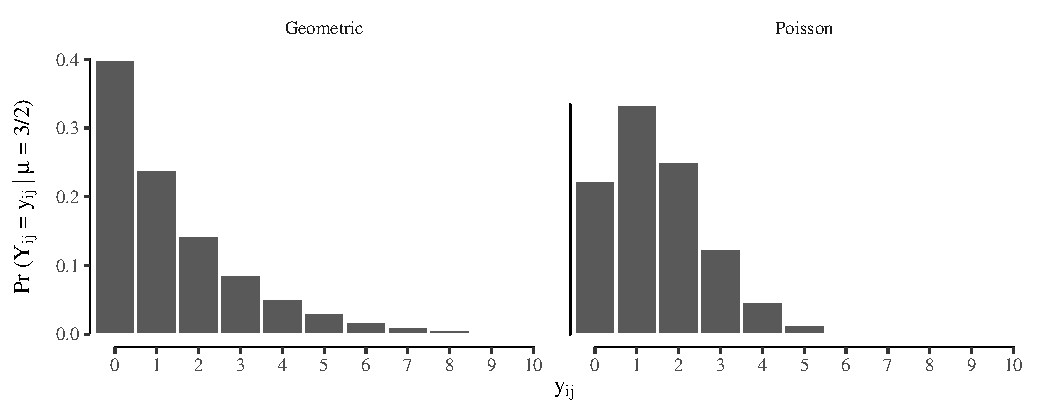
\includegraphics[width=\maxwidth]{figure/geom_pois-1} 

}



\end{knitrout}
\caption [Geometric and Poisson Distribution with Mean = 3.5]{These plots show the shape of Geometric and Poisson Distribution. Both distributions have equal mean, $\mu = \frac{3}{2}$. Differs from Poisson, Geometric Distribution has a strictly decreasing probability as $y_{ij}$ increased.}
\label{fig: Geometric and Poisson}
\end{figure}

On a side note, there is an error in \citet{countergmdefined} on the normalization constant of the 2 distributions above. 
For equation \ref{eq: edgewise Geometric}, \citet{countergmdefined} normalization constant is $\prod_{(i,j) \in \mathbb{Y}}\frac{1}{1-\exp(\theta)}$ when it is supposed to be  $\prod_{(i,j) \in \mathbb{Y}}1-\exp(\theta)$.
Whereas for equation \ref{eq: edgewise Poisson}, the normalization constant is supposed to be $\prod_{(i,j) \in \mathbb{Y}} \me^{-\exp(\theta)}$ instead of $\prod_{(i,j) \in \mathbb{Y}}\frac{1}{\exp(\theta)}$. 
However, these mentioned errors do not affect his conclusion on the respective models.

Besides the Poisson and Geometric Distribution, there are other \textit{reference measures} which corresponds to other \textit{baseline distribution}.
\citet{countergmapplied} introduced \textit{binomial-reference} and \textit{truncated geometric-reference} where it still focus on count edge's value, but there is a cap on the maximum attainable value.  
These constrained models will not  be explored in this paper.

\section{ERGM Count Modelling}
Previously, the form of the ERGM Count was reduced to edge-wise Poisson and Geometric Distribution. 
These two models are rather simple and easily interpreted. 
However, both may not be the model that best fit the later application on Chapter 4.
In addition, these two modes do not take into account the complex relationship of a network.
We will explore more complex models and their interpretations later.

In this section, we will focus on \textit{poisson-reference} ERGM Count without complex constraints: $\mathcal{Y} \in \mathcal{N}_0^{\mathcal{Y}}$ and $h(\bm{y}) = \prod_{(i,j) \in \mathbb{Y}}(y_{ij}!)^{-1}$. 

Furthermore, the linear ERGM Count restriction will also be applied where $\eta(\bm{\theta}) = \bm{\theta}$ and thus $q = p$. 
This restriction makes the model comprehensible. 
In linear ERGM, if $\Theta_{N}$ is an open set, then $\theta_{k}^{\prime} >\theta_{k} \implies E(g_k(\bm{Y})|\theta,\theta_k^{\prime})>E(g_k(\bm{Y})|\theta,\theta_k)$. 
In other words, if other model parameters $\theta \setminus \theta_k$ are fixed, the expected sufficient statistics $g_k$ is strictly increasing in $\theta_k$.
Larger $\theta_k$ will result in a distribution of networks with more feature gauged by $g_k$.

\subsection{Exogenous Covariates}
Let the possibly predictive variables outside the network structure or exogenous covariate be $x_{ijk}$.
A \textit{poisson-reference} ERGM Count will reduce to Poisson Regression Model if we introduce an edge-independent sufficient statistics:
\begin{align}
g_k(\bm{y})= \sum_{(i,j) \in \mathbb{Y}} y_{ij}x_{ijk}.
\end{align}

Let the model sufficient statistics only be exogenous covariate and \BI{sum}  the PMF will reduce to:
\begin{align*}
Pr(\bm{Y}=\bm{y}|\theta) &\propto \frac{\exp\left(\theta_1 \sum_{(i,j) \in \mathbb{Y}} y_{ij} + \theta_k \sum_{(i,j) \in \mathbb{Y}} y_{ij}x_{ijk} \right)}{\prod_{(i,j) \in \mathbb{Y}}y_{ij}!} \\
&= \prod_{(i,j) \in \mathbb{Y}} \frac{(\exp(\theta_1+\theta_k x_{ijk}))^{y_{ij}}}{y_{ij}!}
\end{align*}
This can be recognised as an edge-wise distribution $Y_{ij}\stackrel{\text{iid}}{\sim}\text{poisson}(\lambda =\exp(\theta_1 + \theta_k x_{ijk} ))$ .
Notice that adding exogenous covariate will maintain the poisson relationship yet changing the parameter $\lambda$ for edge $(i,j)$ by multiplication of factor $e^{\theta_k x_{ijk}}$.
It is obvious that further addition of another exogenous covariate will give the same effect.
Hence, this model is equivalent to applying Poisson regression model to the network data.  

In current R implementation of ERGM Count, there can be 3 representation of exogenous covariates for directed network. 
These are \BI{nodeocov} which is the attribute of the actor where the edge originate $x_{i}$ and \BI{nodeicov} which is the attribute of receiving actor $x_j$. 
The last one is $x_{ij}$ or \BI{edgecov} which represent the external edge attribute.

\subsection{Zero Modification}
The idea behind zero modification is to move away from the baseline distribution with new PMF that has more accurate representation of its $Pr(Y_{ij}=0)$. 
The proposed statistics to represent zero modification is \BI{nonzero}:
\begin{align}
g(\bm{y}) = \sum_{(i,j) \in \mathbb{Y}} \mathbb{I}(y_{ij} > 0)
\end{align}
This statistics is simply counting the number of edges that has value bigger than 0. 
Suppose we model ERGM Count that only contain \BI{sum} and \BI{nonzero} statistics. 
Then the PMF will reduce to:
\begin{align*}
Pr(\bm{Y}=\bm{y}|\theta_1,\theta_2) &\propto \frac{\exp\left(\theta_1 \sum_{(i,j) \in \mathbb{Y}} y_{ij} + \theta_2 \sum_{(i,j) \in \mathbb{Y}} \mathbb{I}(y_{ij} > 0)\right)}{\prod_{(i,j) \in \mathbb{Y}}y_{ij}!}\\
&=\prod_{(i,j) \in \mathbb{Y}} \frac{\exp \left(\theta_1 y_{ij} + \theta_2 \mathbb{I}(y_{ij} > 0)\right)}{y_{ij}!}
\end{align*}

This can be recognised as independent edge-wise Zero Modified Poisson, which is a Poisson Distribution with $Pr(Y_{ij}=0)$ can be adjusted by $\theta_2$ while $Pr(Y_{ij}=y_{ij}), y_{ij}=1,2,\ldots,$ maintain their relative proportion.
The corresponding parameter $\theta_2$ can take on any real values. 
If $\theta_2 <0$, then the probability of an edge to take value of zero is higher than Poisson Distribution. 
Whereas if $\theta_2>0$, the number of non-zero edge has higher probability than Poisson Distribution, thus giving the name \textit{\textbf{nonzero}}. Figure \ref{fig: Zero Modified Poisson} will illustrate this relatioship.

\begin{figure}[H]
\begin{knitrout}
\definecolor{shadecolor}{rgb}{0.969, 0.969, 0.969}\color{fgcolor}

{\centering 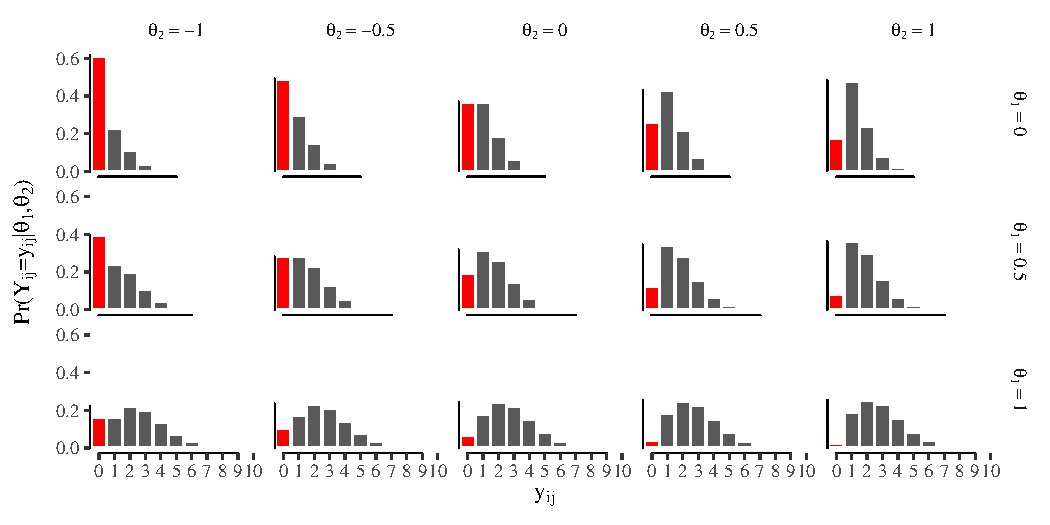
\includegraphics[width=\maxwidth]{figure/unnamed-chunk-2-1} 

}



\end{knitrout}
\caption ["Illustration of Zero-Modified Poisson"]{This figure shows the effect of adding on \textit{\textbf{nonzero}} to the Poisson model. The top axis indicates parameter $\theta_2$, which affect the probability of zero edges. Notice that the effect diminished as parameter $\theta_1$ (right axis) gets higher. Furthermore, $e^{\theta_1}$ is the mean parameter when $\theta_2=0$.}
\label{fig: Zero Modified Poisson}
\end{figure}


\subsection{Dispersion Modelling}
Poisson distribution has only 1 parameter that affect the distribution. This parameter found to affect the mean and the spread of the distribution. For one particular value of mean, there is only one particular spread poisson can attain. In other words, the spread is fixed and not adjustable. The same occurs with other one parameter distributions such as geometric.

One method to overcome this limitation is by adding sufficient statistic,\textit{\textbf{CMP}}:
\begin{align}
g(\bm{y}) = \sum_{(i,j) \in \mathbb{Y}} \log(y_{ij}!)
\end{align}
When only sufficient statistics use in the model is \textit{\textbf{sum}} and \textit{\textbf{CMP}} with poisson reference, the PMF:
\begin{align*}
Pr(\bm{Y}=\bm{y}|\theta_1,\theta_2) &\propto \frac{\exp\left(\theta_1 \sum_{(i,j) \in \mathbb{Y}} y_{ij} + \theta_2 \sum_{(i,j) \in \mathbb{Y}} \log(y_{ij}!)\right)}{\prod_{(i,j) \in \mathbb{Y}}y_{ij}!}\\
&\propto \prod_{(i,j) \in \mathbb{Y}} (\exp(\theta_1))^{y_{ij}} (y_{ij}!)^{\theta_1-1}
\end{align*}
Hence the model reduced to edge-wise \textit{Conway-Maxwell-Poisson} \textit{\textbf{CMP}} distribution $Y_{ij}\stackrel{\text{iid}}{\sim}\text{CMP}(\lambda =\exp(\theta_1),\nu = 1-\theta_2)$ where $\theta_2 \le 1$. When $\theta_2$ goes from 0 to $-\infty$, the distribution become less and less dispersed compare to Poisson. When $\theta_2 \to -\infty$, it is reduced to Bernoulli Distribution. Whereas if as $\theta_2$ from 0 to 1, the distribution is more dispersed compare to Poisson. It is reduced  to Geometric Distribution at $\theta_2=1$. Figure ... will illustrate the various shapes of CMP distribution.

\begin{figure}[H]
\begin{knitrout}
\definecolor{shadecolor}{rgb}{0.969, 0.969, 0.969}\color{fgcolor}

{\centering 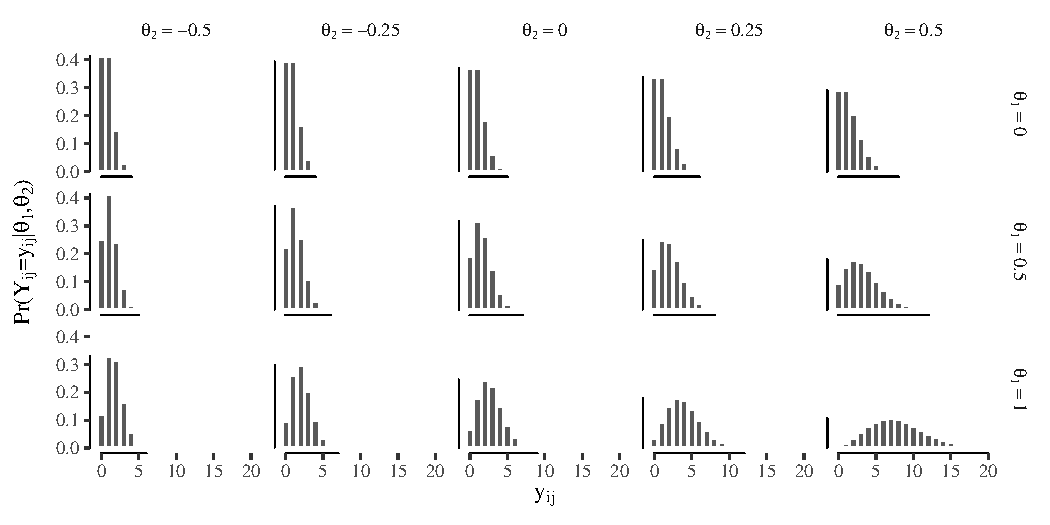
\includegraphics[width=\maxwidth]{figure/unnamed-chunk-3-1} 

}



\end{knitrout}
\caption ["Illustration of Conway-Maxwell-Poisson Distribution"]{This image shows the various shapes of Conway-Maxwell-Poisson Distribution (CMP). The right axis corresponds to parameter $\theta_1$. Whereas the top axis indicates parameter $\theta_2$, which dominates the dispersion effect of the distribution. When $\theta_2 = 0$, CMP reduce to Poisson with mean $e^{\theta_1}$. When $\theta_2 >0$ the distribution become more dispersed, then it gets less dispersed when $\theta_2<0$.}  
\end{figure}


\subsection{Mutuality}
The previous sections discussed the various models that has independent edge-wise assumption. Although, normalization constants tend to be intractable, they can be easily recognised as one particular distribution. However, fitting network data to independent edge-wise model will undermine the inherent relational characteristic of network properties. 

In directed network, the strength of mutuality is one of the network structure that one might consider. In friendship network, mutuality might be defined as when one person claimed to be friend with someone, the opposite party will reciprocate and claim the same. It can also be defined when one declare to be an enemy, the other party also declare the referral to be an enemy. Surely, the tendency to be mutual differs on different network. Hence being mutual in binary network can be defined as $y_{ij}=y_{ji}=1$ or sometimes $y_{ij}=y_{ji}$.

Addition of mutuality will make the ERGM Count model difficult to interpret. Krivitsky suggest that we can understand the model through conditional distribution:
$Pr(Y_{ij}=y_{ij}| \bm{Y} \in \mathcal{Y}_{ij}(y))$ where 
$\mathcal{Y}_{ij}(y)$ is a set where only edge $y_{ij}$ can change it's value where others assumed to be constant.
This means that we will know which value $y_{ij} \in \mathbb{N}_0$ will random variable $Y_{ij}$ likely to attain, given one particular network values. 

However, we will proof that addition of mutuality will reduce to model with independent pair-wise distribution. 
Where a pair represents 2 edges where the origin and destinaton nodes are opposite of each other.
The proposed statistics to represent mutuality are:
\begin{itemize}

\item \textit{\textbf{Minimum}}

One of the proposed statistics to represent mutuality is minimum value or \textit{\textbf{mutual("min")}}: 
\begin{align}
g(\bm{y}) = \sum_{(i,j)\in\mathbb{Y},i<j} \min(y_{ij},y_{ji})
\end{align}
This is simply taking minimum values between 2 opposite edges of a dyad, and sum it for every possible pair.
When a model only use the \textit{\textbf{sum}} and \textit{\textbf{mutual("min")}}, the PMF:
\begin{align*}
Pr(\bm{Y}=\bm{y}|\theta_1,\theta_2) &\propto \frac{\exp\left(\theta_1 \sum_{(i,j) \in \mathbb{Y}} y_{ij} + \theta_{2}\sum_{(i,j)\in\mathbb{Y},i<j} \min(y_{ij},y_{ji})\right)}{\prod_{(i,j) \in \mathbb{Y}}y_{ij}!}\\
&= \frac{\exp\left(\theta_1 \sum_{(i,j) \in \mathbb{Y},i<j} (y_{ij}+y_{ji}) + \theta_{2}\sum_{(i,j)\in\mathbb{Y},i<j} \min(y_{ij},y_{ji})\right)}{\prod_{(i,j) \in \mathbb{Y},i<j}y_{ij}!y_{ji}!}\\
&= \prod_{(i,j) \in \mathbb{Y},i<j} \frac{\exp(\theta_1(y_{ij}+y_{ji})+\theta_2 \min(y_{ij},y_{ji}))}{y_{ij}!y_{ji}!}
\end{align*}
Note that this cant be reduced into edge-wise distribution as per previous sections. Yet it has indendent pair-wise distribution where $\forall(i,j) \in\mathbb{Y},i<j$, the joint distribution of $(Y_{ij},Y_{ji})$ has PMF:
\begin{align*}
P(Y_{ij}=y_{ij},Y_{ji}=y_{ji}|\theta_1,\theta_2) \propto \frac{\exp(\theta_1(y_{ij}+y_{ji})+\theta_2 \min(y_{ij},y_{ji}))}{y_{ij}!y_{ji}!}
\end{align*}

\item \textit{\textbf{Negative Absolute Difference}}

Another proposed statistics is negative absolute difference or \textit{\textbf{mutual("nabsdiff")}} which has the form:
\begin{align}
g(\bm{y}) = \sum_{(i,j)\in\mathbb{Y},i<j} -|y_{ij} - y_{ji}| 
\end{align}
Note that the statistics g's maximum value is 0. 
It is achieved when $\forall(i,j) \in\mathbb{Y},i<j (y_{ij}=y_{ji})$ or every pair is equal. 
The negation of the statistics is necessary as the higher the statistics, the higher strength of mutuality. 
With the same method as above, the pairwise distribution $(Y_{ij},Y_{ji})$ has PMF:
\begin{align*}
Pr(Y_{ij}=y_{ij},Y_{ji}=y_{ji}| \theta_1,\theta_2) \propto \frac{\exp(\theta_1 (y_{ij}+y_{ji}) - \theta_2 |y_{ij}-y_{ji}|)}{y_{ij}!y_{ji}!F} 
\end{align*}

\item \textit{\textbf{Geometric Mean}}

The last proposed statistics is geometric mean or \textit{\textbf{mutual("geomean")}} which has the form:
\begin{align}
g(\bm{y}) = \sum_{(i,j)\in\mathbb{Y},i<j} \sqrt{y_{ij}}\sqrt{y_{ji}} 
\end{align}
Similarly the model with statistics \textit{\textbf{sum}} and \textit{\textbf{mutual("geomean")}} will have independent pairwise ditribution $(Y_{ij},Y_{ji})$ with PMF:
\begin{align*}
Pr(Y_{ij}=y_{ij},Y_{ji}=y_{ji}| \theta_1,\theta_2) \propto \frac{\exp(\theta_1 (y_{ij}+y_{ji}) + \theta_2 \sqrt{y_{ij}}\sqrt{y_{ji}})}{y_{ij}!y_{ji}!} 
\end{align*}
\end{itemize}
Before we discuss the differences of each parameter, it is best to look at the  shapes of the joint distribution. 
\begin{figure}[H]
\begin{knitrout}
\definecolor{shadecolor}{rgb}{0.969, 0.969, 0.969}\color{fgcolor}

{\centering 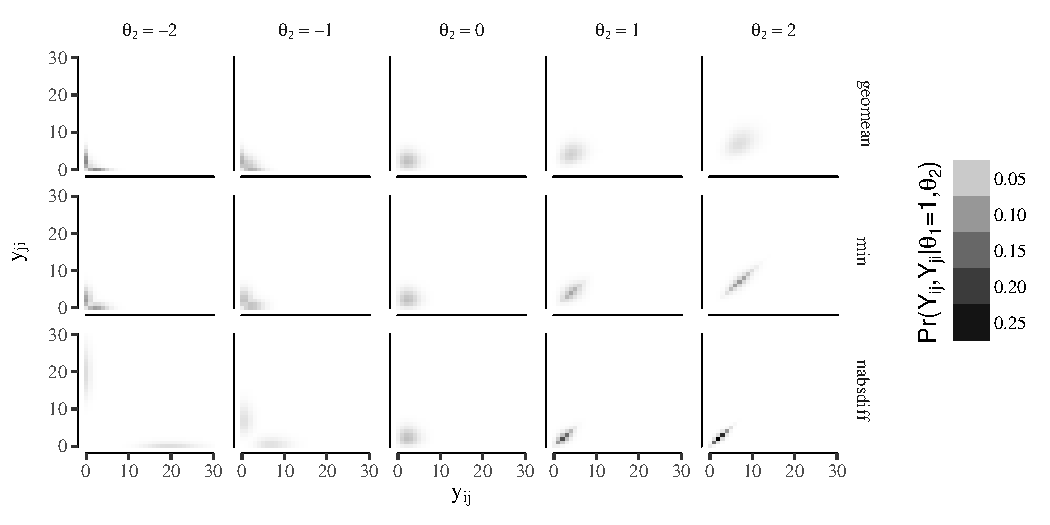
\includegraphics[width=\maxwidth]{figure/unnamed-chunk-4-1} 

}



\end{knitrout}
\caption [Joint distribution with mutual statistics]{This image shows the various PMF of the joint distribution with $\theta_1 =1 $. The different shades of black indicate the region that has higher probability. Here the top axis represent $\theta_2$ which coressponds to the parameter of \textit{\textbf{mutual}} statistics. When $\theta_2 = 0$, the joint distibution follows 2 independent Poisson with $\lambda = e^{\theta_1}$}
\end{figure}

The differences of the joint distributions lies on the dependency statistics $\min(y_ij,y_ji),-|y_{ij}-y_{ji}|, \text{ and} \sqrt{y_{ij}}\sqrt{y_{ji}}$ for 
 \BI{min}, \BI{nabsdiff} and \BI{geomean} respectively.
When $\theta_2>0$ for \BI{min} and \BI{geomean}, the probability will increase as $y_{ij}$ and $y_{ji}$ increase. 
This shifted the distribution to higher pair values. 
For \BI{nabsdiff} the level of $y_{ij}$ and $y_{ji}$ does not affect the reduction of probability. 
However, the reduction occurs less when disparity between $y_{ij}$ and $y_{ji}$ is low and 0 reduction at $y_{ij}=y_{ji}$. 
Hence the distribution is "pulled-in" to the mutual values. 
The same occurs in \BI{min}, such that the highest increase occurs when $y_{ij}=y_{ji}$. 
Hence the distribution is "pulled-up" to mutual values.

When $\theta_2 <0$, \BI{min} and \BI{geomean} will experience higher reduction at higher values of $y_{ij}$ and $y_{ji}$. The reduction stop as $y_{ij}$ or $y_{ji}$ equals to zero. 
Hence, it creates bimodal distribution that has low values with opposing edge has zero value. 
The \BI{min} shows less abrupt clouds as the reduction varies. 
The effect differs significantly from \BI{nabsdiff}. 
There is increase in probability especially when the disparity is high, which creates the bimodal distribution. 
Since now the level of $y_{ij}$ or $y_{ji}$ affect the increase, the distribution cloud clutter on the higher values with opposinge edge is close to 0.

\subsection{Transitivity}
not done
\chapter{Fitting of ERGM}
 
\chapter{Application}
Most of application in ERGM Count has been focusing on social network analysis. 
Whether it is ... and ... 

Here we will fit English Premier League(EPL) data to ERGM COunt.
EPL is the top tier of footbal competition in England.
It is regarded as the world most watched sports league in the world. 

At the first glance, it may not be seem that EPL exhibit a graph representation. We will try to justify the fitting of ERGM Count in the next section.  

\section{Justification ERGM Count Fitting}

In EPL there are 20 teams which represent the nodes of the graph. There will be football matches wehre 2 teams will be playing aginst one another. 
Within 90 minutes period, each team are supposed to score as many goals as possible to the opponent.
At the end of the match the team with the highest accumulated goals will win the match. 
We can then define $y_{ij}$ as the total number of goals scored from team $i$ to team $j$.
The opposing edge $y_{ji}$ will then represent the number of goals from team $i$ to team $j$ in the same match. 
The game may end up in draw if both of the team have equal goals.
On halfway of the league, each team has finished exactly one match against every other team. 
The graph is now complete such that, all the edges combination have probability to attain values other than 0. 
We can then fit ERGM Count to the EPL data.
One example of the graph that will be fitted is shown in Figure \ref{fig:EPL2015}

\begin{figure}[H]
\begin{knitrout}
\definecolor{shadecolor}{rgb}{0.969, 0.969, 0.969}\color{fgcolor}\begin{kframe}


{\ttfamily\noindent\bfseries\color{errorcolor}{\#\# Error in gzfile(file, "{}rb"{}): cannot open the connection}}

{\ttfamily\noindent\bfseries\color{errorcolor}{\#\# Error in plot(nonzero, layout = layout\_in\_circle, vertex.label.dist = 0.8, : object 'nonzero' not found}}

{\ttfamily\noindent\bfseries\color{errorcolor}{\#\# Error in strwidth(legend, units = "{}user"{}, cex = cex, font = text.font): plot.new has not been called yet}}\end{kframe}
\end{knitrout}
\caption [Graph Representation of a Football League]{This is the graph representation of the first half of EPL 2015-2016. The red circles denote the 20 teams that are participating. Its size corresponds to the average market value of the players in the team. The bigger the circle, the average price of the players is higher. The color of the arrow arrow represents total goal scored by the team it orginates from, to the team pointed by the arrow head. The darker the color, the more goals scored in the match. Note that zero total goals scored are omitted.}
\label{fig:EPL2015}
\end{figure}

The interpretation of sufficient statistics will differs significantly from Krivistky's examples. 
First of all, it is unclear whether the goals scored can be modelled with Poisson or Geometric Distribution.
Maybe the \BI{nonzero} or \BI{CMP} distributions may also fit better. 
Here we are interested in finding the best shape of edge-wise distribution.
The notion behind the distribution is not of our interest.
For example, the goals may be well described by Geometric Distribution. 
However, the fact on Geometric Distribution represents the number of trials until the first success is not meaningful in this scenario.

Assuming Poisson Distribution is appropriate, we can further explore the exogenous covariates that may affect the mean. 
As mentioned in Figure \ref{fig:EPL2015}, one of the exogenous covariates is average market value of the players in the team attribute. 
This attribute will be explained further in Data Abstraction Section.
We will also consider whether 
There maybe other covariates that may provide a better fit.
However, as of now these 2 attributes are the only readily available data that is deemed to be appropriate.

Furthermore, we can assess the strength of the \BI{mutuality} of the network with ERGM Count.
Here \BI{mutuality} depicts the tendency for both teams in a match to score the same goals.
This seems to be unlikely as each team main goal is to win the match. 
Whereas the negative or \BI{anti-mutuality} can be interpreted as dominating effect.
When one of the team scores really high, the opposing tends to score low or none at all.
Anecdotal cases show such event may occur. 
We will investigate this effect further in Model Fitting and Analysis section.

The \BI{transitivity} attribute of the network is also interesting. 
If transitivity is found to be significant, when one team scores many goal to other team  

\section{More on The Data}
MOst of the data was retrieved from \textit{www.football-data.co.uk}.
The data files are downloadable csv files with consistent format for every different years.
These includes total goals scored by every team, from every football matches. 
The Home and Away attributes can also be abstracted easily from the files. 
There are many discrepancies in the name of the team with regards to the reality.
As a result, combining with other data source was found to be troublesome and laborious.

However, I managed to manually retrieve other attributes from \textit{www.transfermarkt.com}.
The attribute is the average market value of each player on that team during the particular competition period. 
The derivation of the market value of a player is not fully disclosed.
Users can express their opinion on the value itself.
Experts claim that there is high degree of correlation of the market value with actual sampled salary.
The market value has also been studied by ...

There are 6 complete graph that can be fit to each of different model. The data is summarised by the figure.

\section{Analysis on EPL based on ERGM Count}
\subsection{Analysis on Baseline Distribution}
We would like check whether 




\bibliography{my_bib}{}


\bibliographystyle{apalike}
\end{document}
